\documentclass[noend]{amsproc}

\renewcommand{\arraystretch}{1.3}
\linespread{1}

\usepackage{amsthm,amsmath,amsfonts,mathrsfs,amssymb,lscape,array}
\usepackage{algorithm}
\usepackage{algorithmic}
\usepackage{multirow}
\usepackage{rotating}
\usepackage{enumerate}

\newtheorem{theorem}{Theorem}
\newtheorem{defn}[theorem]{Definition}
\newtheorem{lemma}[theorem]{Lemma}
\theoremstyle{definition}
\newtheorem{remark}[theorem]{Remark}
\newtheorem{example}[theorem]{Example}

% ALGORITHM style
\renewcommand{\algorithmicrequire}{\textbf{Input:}}
\renewcommand{\algorithmicensure}{\textbf{Output:}}

\newcommand{\Singular}{\textsc{Singular}}
\newcommand{\realclassify}{\texttt{realclassify.lib}}
\newcommand{\NF}[1]{\operatorname{NF}(#1)}
\newcommand{\tY}{\widetilde{Y}}

\DeclareMathOperator{\ord}{ord}
\DeclareMathOperator{\requiv}{\overset{r}{\sim}}
\DeclareMathOperator{\m}{\mathfrak{m}}
\DeclareMathOperator{\jt}{jet}
\DeclareMathOperator{\supp}{supp}
\DeclareMathOperator{\sign}{sign}
\DeclareMathOperator{\N}{\mathbb{N}}
\DeclareMathOperator{\Z}{\mathbb{Z}}
\DeclareMathOperator{\Q}{\mathbb{Q}}
\DeclareMathOperator{\R}{\mathbb{R}}
\DeclareMathOperator{\C}{\mathbb{C}}
\DeclareMathOperator{\K}{\mathbb{K}}
\DeclareMathOperator{\A}{\mathbb{A}}
\DeclareMathOperator{\T}{T}
\DeclareMathOperator{\Aut}{Aut}
\DeclareMathOperator{\id}{id}
\DeclareMathOperator{\Quot}{Quot}
\DeclareMathOperator{\dash}{\textnormal{-}}
\DeclareMathOperator{\jet}{jet}
\usepackage{tikz}
\usetikzlibrary{matrix,arrows}

\hyphenation{ne-ces-sary}

\title[The classification of real singularities using \textsc{Singular}, %
Part II]%
{The classification of real singularities using \textsc{Singular}\\
Part II: The Structure of the Equivalence Classes of the Unimodal %
Singularities}

\author{Magdaleen S. Marais}
\address{Magdaleen S. Marais\\
African Institute for Mathematical Sciences and Stellenbosch University\\
6 Melrose Rd\\
Muizenberg 7945, Cape Town\\
South Africa}
\email{magdaleen@aims.ac.za}

\author{Andreas Steenpa\ss}
\address{Andreas Steenpa\ss\\
Department of Mathematics\\
University of Kaiserslautern\\
Erwin-Schr\"odinger-Str.\\
67663 Kaiserslautern\\
Germany}
\email{steenpass@mathematik.uni-kl.de}

\thanks{ }
\subjclass[2000]{}
\keywords{}
\begin{document}
\begin{abstract}
The algorithms implemented in the library ``realclassify.lib" in
\textsc{singular} are discussed in this paper. The purpose of this library is
to classify the~$0$ and $1$ modal isolated hypersurface singularities at $0$ of
corank $0$, $1$ and $2$ over the real numbers as computed by V.I.~Arnold in
\cite{AVG1985}.
\end{abstract}
\maketitle


\section{Introduction}

\begin{table}[tp]
\centering
\caption{Normal forms of singularities of modality $1$ and corank $2$.}
\label{tab:normal_forms}
\begin{tabular}{|c|c|c|c|c|}
\hline

\multicolumn{1}{|c}{}
 & & Complex     & Normal forms     & \multirow{2}{*}{Restrictions} \\
\multicolumn{1}{|c}{}
 & & normal form & of real subtypes &                               \\
\hline\hline


\multirow{6}{*}{\begin{sideways}Parabolic\end{sideways}}

& \multirow{4}{*}{$X_9$} & \multirow{4}{*}{$x^4+ax^2y^2+y^4$}
  & $+x^4+ax^2y^2+y^4$ $(X_9^{++})$ & \multirow{2}{*}{$a^2\neq4$} \\\cline{4-4}
&&& $-x^4+ax^2y^2-y^4$ $(X_9^{--})$ &                             \\\cline{4-5}
&&& $+x^4+ax^2y^2-y^4$ $(X_9^{+-})$ & \multirow{2}{*}{$a^2\neq-4$}\\\cline{4-4}
&&& $-x^4+ax^2y^2+y^4$ $(X_9^{-+})$ &                             \\\cline{2-5}

& \multirow{2}{*}{$J_{10}$} & \multirow{2}{*}{$x^3+ax^2y^2+xy^4$}
  & $x^3+ax^2y^2+xy^4$ $(J_{10}^+)$ & $a^2 \neq 4$ \\ \cline{4-5}
&&& $x^3+ax^2y^2-xy^4$ $(J_{10}^-)$ & -            \\ \hline


\multirow{12}{*}{\begin{sideways}Hyperbolic\end{sideways}}

& \multirow{2}{*}{$J_{10+k}$} & \multirow{2}{*}{$x^3+x^2y^2+ay^{6+k}$}
  & $x^3+x^2y^2+ay^{6+k}$ $(J_{10+k}^+)$
      & \multirow{2}{*}{$a \neq 0,\; k > 0$} \\ \cline{4-4}
&&& $x^3-x^2y^2+ay^{6+k}$ $(J_{10+k}^-)$ &   \\ \cline{2-5}

& \multirow{4}{*}{$X_{9+k}$} & \multirow{4}{*}{$x^4+x^2y^2+ay^{4+k}$}
  & $+x^4+x^2y^2+ay^{4+k}$ $(X_{9+k}^{++})$
      & \multirow{4}{*}{$a \neq 0,\; k > 0$}  \\ \cline{4-4}
&&& $-x^4-x^2y^2+ay^{4+k}$ $(X_{9+k}^{--})$ & \\ \cline{4-4}
&&& $+x^4-x^2y^2+ay^{4+k}$ $(X_{9+k}^{+-})$ & \\ \cline{4-4}
&&& $-x^4+x^2y^2+ay^{4+k}$ $(X_{9+k}^{-+})$ & \\ \cline{2-5}

& \multirow{4}{*}{$Y_{r,s}$} & \multirow{4}{*}{$x^2y^2+x^r+ay^s$}
  & $+x^2y^2+x^r+ay^s$ $(Y_{r,s}^{++})$
      & \multirow{4}{*}{$a \neq 0,\; r,s > 4$} \\ \cline{4-4}
&&& $-x^2y^2-x^r+ay^s$ $(Y_{r,s}^{--})$ &      \\ \cline{4-4}
&&& $+x^2y^2-x^r+ay^s$ $(Y_{r,s}^{+-})$ &      \\ \cline{4-4}
&&& $-x^2y^2+x^r+ay^s$ $(Y_{r,s}^{-+})$ &      \\ \cline{2-5}

& \multirow{2}{*}{$\tY_r$} & \multirow{2}{*}{$(x^2+y^2)^2+ax^r$}
  & $+(x^2+y^2)^2+ax^r$ $(\tY_r^+)$
      & \multirow{2}{*}{$a \neq 0,\; r > 4$} \\ \cline{4-4}
&&& $-(x^2+y^2)^2+ax^r$ $(\tY_r^-)$ &        \\ \hline


\multirow{12}{*}{\begin{sideways}Exceptional\end{sideways}}

& $E_{12}$ & $x^3+y^7+axy^5$ & $x^3+y^7+axy^5$ & - \\ \cline{2-5}

& $E_{13}$ & $x^3+xy^5+ay^8$ & $x^3+xy^5+ay^8$ & - \\ \cline{2-5}

& \multirow{2}{*}{$E_{14}$} & \multirow{2}{*}{$x^3+y^8+axy^6$}
  & $x^3+y^8+axy^6$ $(E_{14}^+)$ & \multirow{2}{*}{-} \\ \cline{4-4}
&&& $x^3-y^8+axy^6$ $(E_{14}^-)$ &                    \\ \cline{2-5}

& $Z_{11}$ & $x^3y+y^5+axy^4$ & $x^3y+y^5+axy^4$ & - \\ \cline{2-5}

& $Z_{12}$ & $x^3y+xy^4+ax^2y^3$ & $x^3y+xy^4+ax^2y^3$ & - \\ \cline{2-5}

& \multirow{2}{*}{$Z_{13}$} & \multirow{2}{*}{$x^3y+y^6+axy^5$}
  & $x^3y+y^6+axy^5$ $(Z_{13}^+)$ & \multirow{2}{*}{-} \\ \cline{4-4}
&&& $x^3y-y^6+axy^5$ $(Z_{13}^-)$ &                    \\ \cline{2-5}

& \multirow{2}{*}{$W_{12}$} & \multirow{2}{*}{$x^4+y^5+ax^2y^3$}
  & $+x^4+y^5+ax^2y^3$ $(W_{12}^+)$ & \multirow{2}{*}{-} \\ \cline{4-4}
&&& $-x^4+y^5+ax^2y^3$ $(W_{12}^-)$ &                    \\ \cline{2-5}

& \multirow{2}{*}{$W_{13}$} & \multirow{2}{*}{$x^4+xy^4+ay^6$}
  & $+x^4+xy^4+ay^6$ $(W_{13}^+)$ & \multirow{2}{*}{-} \\ \cline{4-4}
&&& $-x^4+xy^4+ay^6$ $(W_{13}^-)$ &                    \\ \hline

\end{tabular}
\end{table}
\section{The Sets of Parameter Transformations
$\boldsymbol{P_1}$, $\boldsymbol{P_2}$, and $\boldsymbol{P_3}$}

For the unimodal singularities, we add the values of the parameter which occurs
in the normal form as given in Table~\ref{tab:normal_forms} in parentheses to
the name of the singularity (sub-)type if we want to refer specifically to the
corresponding equivalence class. For instance, we denote by $E_{14}(3)$ the
(complex or real) right-equivalence class of $x^3+y^8+3xy^6$.

For any specific equivalence class $C$, we denote by $\NF{C}$ its normal form
as shown in Table~\ref{tab:normal_forms}, i.e.\@ we write
$\NF{E_{14}(a)} = \NF{E_{14}^+(a)}$ for the polynomial $x^3+y^8+axy^6$ and
$\NF{E_{14}^-(a)}$ for $x^3-y^8+axy^6$.

\begin{defn}
Let $\K$ be either $\R$ or $\C$, let $f,g\in\K[[x_1, \ldots, x_n]]$ and let $S$
be a subset of the set of the $\K$-algebra automorphisms
of $\K[[x_1, \ldots, x_n]]$, i.e.~$S\subset\Aut_{\K}\K[[x_1,\ldots,x_n]]$.
\begin{enumerate}
\item We denote the set of all automorphisms in $S$ which take $f$ to $g$ by
$\T_{\K}^S(f,g)$, i.e.\@
\[
\T_{\K}^S(f,g):=\{\phi\in S\mid \phi(f)=g\}\,.
\]
\item If $S=\Aut_{\K}(\K[[x_1,\ldots,x_n]]$ we only write $\T_{\K}(f,g)$,
i.e.\@
\[
\T_{\K}(f,g)
:= \{\phi \in \Aut_{\K}(\K[[x_1, \ldots, x_n]]) \mid \phi(f) = g \} \,.
\]
\item If $\T_{\K}(f,g)\neq\varnothing$, we write $f\overset{\K}\sim g$.
\end{enumerate}
\end{defn}

\begin{remark}
Let $\K$ be either $\R$ or $\C$. As usual, we denote the quotient field
$\Quot(\K[a])$ by $\K(a)$. Let $f \in \K(a)[[x_1,\ldots,x_n]]$ be a power
series over this quotient field. Then $f$ can be written as
$f = \sum_{\nu \in \N^n} c_\nu \boldsymbol{x}^\nu$ with coeffients
$c_\nu = \frac{p_\nu}{q_\nu} \in \K(a)$ where $p_\nu, q_\nu \in \K[a]$ are
polynomials and $q_\nu \neq 0$ for $\nu \in \N^n$.

If we consider the polynomials $p_\nu, q_\nu$ as polynomial functions
$p_\nu, q_\nu: \; \K \rightarrow \K$, then we may also consider the
coefficients $c_\nu$ as functions
$c_\nu: \; \K \setminus V(q_\nu) \rightarrow \K$ where $V(q_\nu)$ is the set of
points where $q_\nu$ vanishes. Via this correspondence, we finally get power
series
$f(u) := \sum_{\nu \in \N^n} c_\nu(u) \boldsymbol{x}^\nu
\in \K[[x_1,\ldots,x_n]]$ for each value
$u \in \K \setminus \bigcup_{\nu \in \N^n} V(q_\nu)$.

Note that the notation $f(u)$ is compatible with the notations for equivalence
classes and normal forms introduced above in the sense that, e.g.,
$\NF{E_{14}(a)}(b) = \NF{E_{14}(b)}$.
\end{remark}

\begin{defn}
\phantom{X}\hfill
\begin{enumerate}
\item
Given power series $f,g \in \C(a)[[x_1,\ldots,x_n]]$, we define the
first set of parameter transformations of $f$ and $g$ as
\begin{align*}
P_1(f, g)
:= \{ (u, v) \in \C^2 \mid
&f(u) \text{ and } g(v) \text{ are well-defined and } \\
&\T_{\C}(f(u), g(v)) \neq \varnothing \} \,.
\end{align*}

\item
Given power series $f,g \in \R(a)[[x_1,\ldots,x_n]]$, we define the
second set of parameter transformations of $f$ and $g$ as
\begin{align*}
P_2(f, g)
:= \{ (u, v) \in \R^2 \mid
&f(u) \text{ and } g(v) \text{ are well-defined and } \\
&\T_{\C}(f(u), g(v)) \neq \varnothing \} \,.
\end{align*}

\item
Given power series $f,g \in \R(a)[[x_1,\ldots,x_n]]$, we define the
third set of parameter transformations of $f$ and $g$ as
\begin{align*}
P_3(f, g)
:= \{ (u, v) \in \R^2 \mid
&f(u) \text{ and } g(v) \text{ are well-defined and } \\
&\T_{\R}(f(u), g(v)) \neq \varnothing \} \,.
\end{align*}
\end{enumerate}
\end{defn}

\begin{remark}
\phantom{X}\hfill
\begin{enumerate}
\item
Note that $P_3(f, g) \subseteq P_2(f, g) \subseteq P_1(f, g)$ for any two power
series $f,g \in \R(a)[[x_1,\ldots,x_n]]$.

\item
For any two unimodal singularity (sub-)types $T_1, T_2$, we simply write
$P_i(T_1,T_2)$ instead of $P_i(\NF{T_1(a)}, \NF{T_2(a)})$, e.g., we write
$P_1(E_{14}, E_{14})$ for $P_1(\NF{E_{14}(a)}, \NF{E_{14}(a)})$.
\end{enumerate}
\end{remark}

It turns out that in some cases, the sets $P_1$, $P_2$ and $P_3$ are just
unions of sets of the form $(a, ra)_{a \in \K}$ for some $r \in \C$ and $\K$
either $\C$ or $\R$. For those cases we use the following auxiliary notation.

\begin{defn}
For any polynomial $p(X) \in \C[X]$, we define the sets $C(p(X))$ and $R(p(X))$
as
\begin{align*}
C(p(X)) &:= \{ (a, ra) \in \C^2 \mid a, r \in \C, \; p(r) = 0 \} \,, \\
R(p(X)) &:= \{ (a, ra) \in \R^2 \mid a, r \in \R, \; p(r) = 0 \} \,.
\end{align*}
\end{defn}

\begin{defn}
For $\Omega \subset \C$, let $(f_i: \Omega \rightarrow \C)_{i \in I}$ be a
family of complex-valued functions on $\Omega$. We define the joint graph of
$(f_i)_{i \in I}$ as
\[
\Gamma_\Omega((f_i)_{i \in I})
:= \{ (a, f_i(a)) \in \Omega \times \C \mid a\in \Omega,\; i \in I \}\,.
\]
\end{defn}


\section{Finite Jets of Power Series and Transformations}

For background regarding the definitions in this section we refer to
\cite{A1975}.

\begin{remark}
\phantom{X}\hfill
\begin{enumerate}[(a)]
\item Let $\K$ be either $\R$ or $\C$. Throughout this paper we choose weights
$w$ on the variables in $\K[[x_1,\ldots,x_n]]$ such that the weighted degree of
$x_i$, $w\dash\deg(x_i),\ \forall i$ are natural numbers.
\item For $f,g\in\K[[x_1,\ldots,x_n]]$, we mean by $f*_wg$,
$w\dash\deg(f)*w\dash\deg(g)$, where $*$ is any one of $<,\le,>,\ge,=$. We
denote the weighted
$j\dash\jet$ of a power series $f$ by $j\dash w\dash\jet(f)$.
\end{enumerate}
\end{remark}

\begin{defn}
A power series has filtration $d$ if all its monomials are of weighted degree
$d$ or higher. The power series of filtration $d$ form a linear space $E_d^w$.
\end{defn}

\begin{remark}
Note that $E_{d'}^w\subseteq E_d^w$ if $d<d'$. Since the filtration of a
product, $E_{d'}^w\cdot E_d^w$, is the sum of the filtrations of the factors,
$d'+d$, it follows that $E_d^w$ is an ideal in the ring of power series. We
denote the ideal of $E_d^w$ consisting of series of filtration strictly greater
than $d$ by $E_{>d}^w$. If the weight of all the variables are $1$ we only
write $E_d$.
\end{remark}

\begin{defn}\label{phi}
Let $\K$ be either $\R$ or $\C$. Let $\phi$ be an $\K$-algebra automorphism of
$\K[[x_1,\ldots,x_n]]$ and let $w$ be a chosen weight on the variables.
\begin{enumerate}[(a)]
\item For $j > 0$ we define the
\emph{$j$-$w$-jet} of $\phi$, denoted by $\phi_j^w$, to be the automorphism
given by
\[
\phi_j^w(x_i) := w\dash\jet(\phi(x_i),w\dash\deg(x_i)+j) \quad
\forall i = 1,\ldots,n \,.
\]
If the weight of all the variables are $1$, we only write $\phi_j$.\\
\item $\phi$ has filtration $d$ if, $\forall\lambda$,
\[(\phi-1)E_\lambda^w\subset E_{\lambda+d}^w.\]
\end{enumerate}
\end{defn}

\begin{remark}
Note that $\phi_0(x_i)=\jet(\phi(x_i),1)\ \forall i$. Furthermore note that
$\phi_0^w$ has filtration $\le 0$ and, for $j>0$, if $\phi_{j-1}^w=1$, then
$\phi_j^w$ has filtration $j$.
\end{remark}

The infinitesimal analogue of Definition \ref{phi}(2) is:

\begin{defn}
Let $\K$ be either $\R$ or $\C$. A formal vector field
$v=\sum_i v_i\frac{\partial}{\partial x_i}$ over $\K[[x_1,\ldots,x_n]]$, where
$v_i\in\K[[x_1,\ldots,x_n]]$, has filtration $d$ if the directional derivitive
raises the filtration by not less than $d$, i.e.\@
$L_vE^w_\lambda\subset E^w_{\lambda+d}$, where
$L_v(f)=\sum_i v_i\frac{\partial f}{\partial x_i}$.
\end{defn}

\begin{remark}
Throughout the paper we also use the concepts of semi-quasihomo-genious power
series and their quasihomogenious part as well as piecewise quasihomogenious
power series and their Newton polygons. For background regarding these concepts
we again refer to \cite{A1975}.
\end{remark}

\section{Sufficient Sets of Transformations Between Real Normal Forms}
The results in this section narrow down the transformations we need to consider
between specific unimodal normal forms of the same main type, to determine
equivalence, considerably. In fact these results are in many cases the main
step in determining the structure of the equivalence classes of corank 2,
unimodal singularities of the same main type. (See
Section~\ref{OnTheComputationOfTheResults}.)

\begin{defn}
Let $\mathbb L$ and $\K$ both be either $\R$ or $\C$, such that
$\mathbb L\subset\mathbb K$, and let $f,g\in\mathbb L(a)[[x_1,\ldots,x_n]]$. We
call $S\subset \Aut_{\K}(\K[[x_1,\ldots,x_n]])$ a sufficient set of
$\K$-transformations preserving $\mathbb L$ for $f$ and $g$, if for all
$u,v\in\mathbb L$,
\[
T_{\K}(f(u),g(v))\neq\varnothing\Leftrightarrow
\T_{\K}^S(f(u),g(v))\neq\varnothing\,.
\]
\end{defn}
We need the following result to prove the main result of this section,
Theorem~\ref{tab:sufficient_sets}.

The following result is proven in \cite{A1975}.
\begin{lemma}\label{vectorlemma}
Let $\K$ be either $\R$ or $\C$. Let $f=f_0+f_1+f_2\in\K[[x_1,\ldots,x_n]]$,
where $f_0\in E^w_d$, $f_1\in E^w_{>d}$ and $f_2\in E^w_{d+\delta}$, and let
$\phi$ be a $\K$-algebra automorphism defined by
$\phi(x_i)=x_i+v_{0,i}+v_{1,i}$, where
$v_0=\sum_iv_{0,i}\frac{\partial}{\partial x_i}$ has filtration $\delta$ and
$v_1=\sum_iv_{1,i}\frac{\partial}{\partial x_i}$ has filtration strictly
greater than $\delta$ where $\delta>0$. Then
\[
\phi(f)=f_0+\left[ f_1+\sum_iv_{0,i}\frac{\partial f_0}{\partial x_i}\right]+R,
\]
where $R\in E^w_{>d+\delta}$.
\end{lemma}


\begin{theorem}\label{tab:sufficient_sets}\label{thm:sufficient_sets}
Let $\K$ and $\mathbb L$ be either $\R$ or $\C$, respectively, with
$\mathbb L\subset \K$ and let $T_1,T_2$ be two singularity subtypes such that
both are of one of the following main types:
\begin{enumerate}[(a)]
\item[(i)] $J_{10}\,,$
\item[(ii)] $E_{12},E_{13},E_{14},Z_{11},Z_{12},Z_{13},W_{12},W_{13}\,,$
\item[(iii)] $ J_{10+k}\,,$
\item[(iv)] $X_{9+k}\,,$
\item[(v)] $Y_{r,s}\,.$
\end{enumerate}
In the case (i) the set $S_0$, in the cases (ii), (iii) and (iv) the set $S_1$
and in the case (v) the set $S_2$ is, respectively, a sufficient set of
$\K$-transformations preserving $\mathbb L$ for $T_1$ and $T_2$:
\begin{eqnarray*}
S_0&=&\left\{\phi\in\Aut_{\K}(\K[[x,y]])\left |
\begin{array}{l}
\phi(x)=\alpha x+cy^2,\\
\phi(y)=ty, \alpha,c,t\in\K\ (\textit{if $\K=\R$ then $\alpha=1$})
\end{array}
\right.\right\};\\\\
S_1&:=&\{\phi\in\Aut_{\K}(\K[[x,y]])
\mid \phi(x)=\alpha x, \phi(y)=\beta y, \alpha, \beta\in\K\};\\\\
S_2&:=&\left\{\phi\in\Aut({\K}[[x,y]]) \left |
\begin{array}{ll}
\begin{array}{l}
\phi(x)=\alpha x,\quad \phi(y)=\alpha y,\ \alpha,\beta\in\K
\end{array}
&, \textit{ if $r\neq s$}\\\\
\begin{array}{ll}
\phi(x)=\alpha x,& \phi(y)=\beta y,\ \alpha,\beta\in\K\\&\textit{or}\\
\phi(x)=\alpha y,& \phi(y)=\beta x,\ \alpha,\beta\in\K
\end{array}
&,\textit{if $r=s$}
\end{array}
\right.\right\}.
\end{eqnarray*}
\end{theorem}
\begin{proof}

(i) Let $T_1$ and $T_2$ be (not neccesarily different) subtypes of $J_{10}$ and
let $f=T_1(a)$, $a\in\K$. We choose a weight $w$ such that the terms on the
diagonal defined by $f$ have the same weight. Let $\phi$ be a $\K$-algebra
automorphism such that $\phi(f)=T_2(a')$, $a'\in\K$. Using Proposition 6 in
\cite{MS2013}, it follows that $\phi_0(x)=\alpha x$ ($\alpha=1$ if $\K=\R$),
$\alpha\in\K$. Hence $\phi_0^w(x)=\alpha x+cy^2$ and $\phi_0^w(y)=ty$,
$\alpha,c,t\in\K$. Since we only consider terms on the diagonal of $\phi(f)$,
we only need to consider $\phi_0^w(f)$.

(i) We only give the proof for the $E_{12}, E_{13}$ and $E_{14}$ singularities.
The result can be similarly proved for the other Exceptional unimodal cases.
Let $T_1$ be a real $E_{12}$, $E_{13}$ or $E_{14}$ subtype and let $f=T_1(a)$,
$a\in\K$. Then $f$ can be written as $f=f_0+f_1$, where $f_0$ is the sum of the
terms not having the chosen value of the parameter as coefficient and $f_1$ is
the term that has the chosen value for the parameter as coefficient. We choose
a weighted degree $w$ such that the terms of $f_0$ have the same degree $w_0$.
Hence $f_0$ is the quasihomogeneous part of $f$.

Let $\phi$ be a $\K$-algebra automorphism such that $\phi(f)=T_2(a')$,
$a'\in\K$ and $T_2$ a subtype of the same main type as $T_1$.

Note that in this case
\begin{equation}\label{c}
x^2>_w xy >_w y^3>_w x>_w y^2>_w y.
\end{equation}
Let $k_0$ be the degree of lowest jet of $f$, i.e.~$\jet(f,k_0-1)=0$ and
$\jet(f,k_0)\neq 0$. Since

\begin{equation}
\phi(f) = \phi_0(\jet(f,k_0))+\phi_0(f-\jet(f,k_0))+\phi^*(f)
= \phi_0(\jet(f,k_0))+R,\label{lowestjet}
\end{equation}
where $\phi^*=\phi-\phi_0$ and $R\in E_{>k_0}$, it is clear that

\begin{equation}
\phi_0(x)=\alpha x,\quad 0\neq\alpha\in\K,\label{transx}
\end{equation}

i.e~ $\phi_0^{w}(x)=\alpha x$ and $\phi_0^{w}(y)=\beta y$, $\alpha,\beta\in\K$.

Now, $\phi=\phi''\circ\phi'$, where $\phi'$ and $\phi''$ are, respectively,
defined by
\[
\phi'(x)=\alpha x,\quad \phi'(y)=\beta y, \quad
\phi''(x)=\frac{1}{\alpha}\phi(x), \quad\phi''(y)=\frac{1}{\beta}\phi(y).
\]
If $\alpha,\beta\neq 1$, we replace $f$ by $\phi'(f)$ and $\phi$ by $\phi''$
for the following arguments showing that the coefficient of $y^2$ and $y^3$ in
$\phi(x)$, or equivalently $\phi''(x)$, is zero. Taking the ordering in
(\ref{c}) into account, we have that
\[
\phi_0^w(x)=x+cy^2, \quad\phi_0(y)=y,\quad c\in\K.
\]
Note that $\phi^w_0$ has filtration $<0$ if $c\neq 0$, and that
$\phi-\phi^w_0+1$ has filtration $>0$. Furthermore note that
$\phi_0^w(f_1)\in E_{w_0}^w$ in all three cases. Hence,
\begin{eqnarray*}
\phi(f)&=&\phi_0^w(f)+(\phi-\phi^w_0)(f)\\
&=& R_1+c\frac{\partial f_0}{\partial x}y^2+f_0+\phi^w_0(f_1)+R_2
+(\phi-\phi^w_0)(f)=R_1+c\frac{\partial f_0}{\partial x}y^2+R_3,
\end{eqnarray*}
$R_1\in\K[[x,y]]
\setminus E^w_{w\dash\deg\left(\frac{\partial f_0}{\partial x}y^2\right)}$,
$R_2\in E^w_{>w_0}$ and $R_3\in E^w_{w_0}$. Therefore $c=0$ and $\phi$ has
positive filtration.
By (\ref{c}), it follows that
\begin{equation*}
\frac{\partial f_0}{\partial y}x >_w\frac{\partial f_0}{\partial y}y^2
=_w \frac{\partial f_0}{\partial x}xy>_w f_1\quad
\textnormal{and}\quad \frac{\partial f_0}{\partial x}y^3>_w f_0.
\end{equation*}
Therefore, it follows from Lemma \ref{vectorlemma} that
\begin{equation*}
\phi(f) = f_0+c\frac{\partial f_0}{\partial x}y^3+f_1+R,\quad
R\in E^w_{>w\dash\deg(\frac{\partial f_0}{\partial x}y^3)}
\end{equation*}
where $\phi(x) = x+ cy^3+R'$, $R'\in E^w_{>w\dash\deg(y^3)}$, $c\in\K$. If
$f_1\in E^w_{>w\dash\deg(\frac{\partial f}{\partial x}y^3)}$ then it follows
that $c=0$ and we apply Lemma \ref{vectorlemma} again, this time with
$\phi(x)=x+cy^4+R'$, where $R'\in E^w_{>w\dash\deg(y^4)}$, $c\in\K$. Since
$\gamma_0\frac{\partial f_0}{\partial x}y^n+\gamma_1f_1\neq \gamma_2f_1$ for
any $\gamma_0,\gamma_1,\gamma_2\in\K$, $n\in\N$, $\gamma_0\neq 0$, in all three
cases, the result follows.

(ii) Let $T_1$ be the subtype $J_{10+k}^+$ or the subtype $J_{10+k}^-$ and let
$f=T_1(a)$, $a\in\K$.
The Newton polygon defined by the principal part $f_0=x^3\pm x^2y^2+ay^{6+k}$,
$a\in\K$, of $f$ has two faces. Choose weights $w_1$ and $w_2$ for the two
faces defined by $f_{1,0}=x^3\pm x^2y^2$ and $f_{2,0}=x^2y^2+ay^{6+k}$ such
that all the terms on the two faces have the same weight $k_0$. We denote the
piecewise weight by $k_0$. We refer to the terms above the two faces,
respectively, as $f_{1,1}=ay^{6+k}$ and $f_{2,1}=x^3$.

Let $\phi$ be a $\K$-algebra automorphism that transforms $f$ to $T_2(a')$,
where $a'\in\K$ and $T_2$ is a subtype of the same main type as $T_1$.

Considering the $3$-jet of $f$ it follows that $\phi_0(x)=\alpha x$. Hence
$\phi_0^{w_1}(x)=\alpha x+cy^2$ and $\phi_0^{w_1}(y)=\beta y$,
$\alpha,c,\beta\in\C$, $\alpha,\beta\neq 0$, which implies that $\phi^{w_1}_0$
has non-negative filtration with regard to the weight $w_1$. Hence
\begin{eqnarray*}
\phi(f)&=&\phi^{w_1}_0(f)+(\phi-\phi^{w_1}_0)(f)\\
&=&\alpha^3x^3+\alpha^2(3c\pm\beta^2)x^2y^2+\alpha(3c^2\pm2 c\beta^2)xy^4
+(c^3\pm c^2\beta^2)y^6+R,
\end{eqnarray*}
where $R\in E^{w_0}_{>k_0}$. Since $\phi(f)$ is of type $J_{10+k}$, $c$ is a
root of $k(z)=z^3\pm z^2\beta^2$ and $k'(z)=3z^2\pm2 z\beta^2$. Hence $c=0$.

Since $\phi-\phi_0^{w_1}+1$ has positive filtration with regard to $w_1$ it
follows that
\begin{equation}\label{transw2}
\phi(f) = \phi_0^{w_1}(f_1) + R,\quad R\in E^{w_1}_{>k_0}.
\end{equation}
Note that
\begin{equation}\label{orderw1}
y<_{w_2}x<_{w_2}xy^n,
\end{equation}
for all $n\ge 1$. We, now, consider recursively the next smallest $s>2$ such
that $y^s<_{w_2}x$. Note that $\phi_0^{w_2}(x)=x+cy^s+R$,
$R\in E^{w_2}_{>w_2\dash deg(y^2)}$. Therefore if $c\neq 0$, then
$\phi_0^{w_2}$ has negative filtration with regard to the weight $w_2$ and
$\phi-\phi_0^{w_2}+1$ has positive filtration. Because $s>2$ it follows that
$w_2\dash\deg(y^sx^2)>k_0$ and that $y^{2s}x>_{w_2}y^{s+2}x$. Since
$y^s<_{w_2}x$ it follows furthermore that
$w_2\dash\deg(y^{s+2}x)<w_2\dash\deg(x^2y^2)=k_0$. Hence
\begin{eqnarray*}
\phi(f) &=& \phi_0^{w_2}(f)+(\phi-\phi_0^{w_2})(f)\\
&=& R_1+2\beta^2\alpha c xy^{s+2}+\phi_0^{w_2}(f_{2,1})+R_2\\
&=&R_1+2\beta^2\alpha c xy^{s+2}+ 3 c^3y^{3s}+ 3\alpha c^2y^{2s}x
+3\alpha^2 cy^sx^2+R_2\\
&=&R_1+2\beta^2\alpha c xy^{s+2}+ 3c^3y^{3s}+R_3,
\end{eqnarray*}
where $R_1\in\K[[x,y]]\setminus E^{w_2}_{w_2\dash\deg(xy^{s+2})}$,
$R_2, R_3\in E^{w_2}_{>w_2\dash\deg(xy^{s+2})}$. Therefore $c=0$ and
$\phi_0^{w_2}(x)=x$ and $\phi_0^{w_2}(y)=\beta y$. Thus $\phi$ has non-negative
filtration with regard to $w_2$ and
\begin{equation}\label{transw1}
\phi(f) = \phi_0^{w_2}(f_2)+R,\quad R\in E^{w_2}_{>k_0}.
\end{equation}
Now, it follows from (\ref{transw2}) and (\ref{transw1}) that
\begin{equation*}
\phi(f) = \phi_0^{w_0}(f_0)+R,\quad R\in E^{w_0}_{>k_0}.
\end{equation*}
Since $\phi(f)$ is again of main type $J_{10+k}$, it follows that
\begin{equation*}
\phi(f) = \phi_0^{w_0}(f_0)=\phi_0^{w_0}(f).
\end{equation*}

(iii) and (iv) follows similar to (ii).

(v) Let $T_1(a)=\sigma(x^2+y^2)^2+ax^r$ and $T_2(a')=\sigma'(x^2+y^2)^2+a'x^r$,
where $a,a'\in\K$, $\sigma=\pm 1$ and $\sigma'=\pm\sigma$, and, $T_1$ and $T_2$
(not necessarily different) subtypes of $\widetilde Y_{r}$. Suppose there
exists a $\phi^T\in\T_{\K}(T_1,T_2)$ such that $\phi^T(T_1(a))=T_2(a')$.
\end{proof}


\section{On the Computation of the Results}\label{OnTheComputationOfTheResults}

Based on the previous section, all of the results presented in
Section~\ref{sec:results} can be computed using \Singular{}. The main tools for
these computations are elimination, Gr\"obner covers, and primary
decomposition. For each pair of singularity subtypes~$T_1, T_2$, the
computation follows the same structure: One can first compute the set
$P_1(T_1, T_2)$ using elimination and factorization. The set $P_2(T_1, T_2)$
can then be derived from this as the intersection of $P_1(T_1, T_2)$ with
$\R \times \R$. In order to determine $P_3(T_1, T_2)$, one finally has to check
for each point or branch in $P_2(T_1, T_2)$ whether or not there is a real
transformation which changes the parameter in such a way. Gr\"obner covers and
primary decomposition are convenient tools to simplify the often complicated
ideals which occur in this last step.

Although our approach is almost algorithmic, we do not present it as an
algorithm here because each case requires slightly different means depending on
the intermediate results. Especially the computation of $P_3(T_1, T_2)$ is
rather straighforward in some cases whereas it requires careful considerations
in other cases.

However, writing down every detail of the computations for each case is beyond
the scope of this section. Instead, we will present the general framework and
give explicit \Singular{} commands for $T_1 = T_2 = X_9^{++}$ which is one of
the more complicated cases (cf. Theorem~\ref{thm:X9}).


\subsection{How to compute $\boldsymbol{P_1(T_1, T_2)}$}%
\label{sec:computing_P1}

Let $S \subset \Aut_{\C}(\C[[x,y]])$ be the sufficient set of
$\C[[x,y]]$-automorphisms for $T_1$ and $T_2$ given in
Theorem~\ref{thm:sufficient_sets}. Then $S$ can be covered by an automorphism
$\phi \in \Aut_{\C}(\C[[x,y]])$ with generic coefficients $t_1, \ldots, t_r$,
i.e.\@ by a $\phi$ of the form $\phi(x) = t_1 \cdot x + (\text{other terms})$
where for any element $\psi \in S$, one can plug in specific values for
$t_1, \ldots, t_r$ such that $\psi = \phi$.

Let us denote the parameter occurring in $T_1$ by $a$ and the one in $T_2$ by
$b$. By comparing the coefficients in $\phi(T_1(a))$ and $T_2(b)$, we get a set
of equations in $a, b, t_1, \ldots, t_r$ which is equivalent to
$\phi(T_1(a)) = T_2(b)$. Let $I \subset \C[a,b,t_1,\ldots,t_r]$ be the ideal
generated by these equations. Then the vanishing set $V(I)$ describes
completely which transformations take $T_1(a)$ to $T_2(b)$ for which values of
$a$ and $b$.

We can now eliminate the variables $t_1, \ldots, t_r$ from $I$ and thus obtain
an ideal $I' \subset \C[a,b]$ which is in all cases generated by one polynomial
$g$. This elimination geometrically corresponds to the projection
$\A_{\C}^{2+r} \supset V(I) \mapsto V(I') \subset \A_{\C}^2$. After factorizing
$g \in \C[a,b]$ into irreducible factors $g_1, \ldots, g_s$, we compute the
roots in $b$ of each factor (over $\C(a)$ or suitable extensions thereof if
necessary). We thus get roots of the form $b-f(a)$ where $f(a)$ can be
considered as a function in $a$. These functions explicitly determine the
possible values of $b$ for each given $a$ and their joint graph is exactly
$P_1(T_1, T_2)$.

\begin{example}\label{ex:P1}
We compute $P_1(X_9^{++}, X_9^{++})$ with Singular. For convenience we work
over $\Q(a,b,t_1,t_2,t_3,t_4)[x,y]$:
\begin{verbatim}
> ring R = (0,a,b,t1,t2,t3,t4), (x,y), dp;
> poly f = x^4+a*x^2*y^2+y^4;
\end{verbatim}
According to Theorem~\ref{thm:sufficient_sets},
\[
S = \{ \phi \in \Aut_{\C}(\C[[x,y]])
\mid \phi(x) = t_1 x + t_2 y,\; \phi(y) = t_3 x + t_4 y,\;
t_1, \ldots, t_4 \in \C \}
\]
is a sufficient set of automorphisms for $X_9$:
\begin{verbatim}
> map phi = R, t1*x+t2*y, t3*x+t4*y;
> matrix C = coef(phi(f), xy);
> print(C);
x^4,   x^3*y, x^2*y^2,x*y^3, y^4,  
C[2,1],C[2,2],C[2,3], C[2,4],C[2,5]
> C[2,1];
(a*t1^2*t3^2+t1^4+t3^4)
\end{verbatim}
Now the second row of the matrix \verb+C+ contains the coefficients of
$\verb+phi+(X_9^{++}(a))$, e.g.\@ \verb+C[2, 1]+ is the one belonging to $x^4$.
Using the corresponding coefficients of
$X_9^{++}(b) = x^4 + b \cdot x^2 y^2 + y^4$, we can define the ideal $I$ as
above:
\begin{verbatim}
> matrix D[1][5] = 1, 0, b, 0, 1;
> ideal I = C[2,1..5]-D[1,1..5];
\end{verbatim}
As the next step, we map this ideal to $\Q(a)[b,t_1,t_2,t_3,t_4]$ and eliminate
the variables~$t_i$:
\begin{verbatim}
> ring S = (0,a), (b,t1,t2,t3,t4), dp;
> ideal I = imap(R, I);
> ideal g = eliminate(I, t1*t2*t3*t4);
> g;
g[1]=(a^4-8*a^2+16)*b^6+(-a^6-720*a^2-1152)*b^4
+(8*a^6+720*a^4+20736)*b^2+(-16*a^6+1152*a^4-20736*a^2)
\end{verbatim}
Factorizing the single generator of this ideal finally yields the functions
$f_1^{1,1}, \ldots, f_6^{1,1}$ defined in Theorem~\ref{thm:X9}. Note that
$a^2 \neq 4$.
\begin{verbatim}
> factorize(g[1]);
[1]:
   _[1]=1
   _[2]=b+(-a)
   _[3]=b+(a)
   _[4]=(a-2)*b+(-2*a-12)
   _[5]=(a+2)*b+(-2*a+12)
   _[6]=(a+2)*b+(2*a-12)
   _[7]=(a-2)*b+(2*a+12)
[2]:
   1,1,1,1,1,1,1
\end{verbatim}
\end{example}


\subsection{How to compute $\boldsymbol{P_2(T_1, T_2)}$}

Given $P_1(T_1, T_2)$, it is easy to compute $P_2(T_1, T_2)$ even ``by hand''
because we have $P_2(T_1, T_2) = P_1(T_1, T_2) \cap (\R \times \R)$.

\begin{example}\label{ex:P2}
Continuing the example above, the values of
$f_1^{1,1}(a), \ldots, f_6^{1,1}(a)$ are clearly real for $a \in \R$, cf.\@
Theorem~\ref{thm:X9}. The set $P_2(X_9^{++}, X_9^{++})$ is thus the joint graph
of these functions over $\R \setminus \{-2, 2\}$.

To give another example, for $T_1 = T_2 = X_9^{+-}$ the set $P_1(T_1, T_2)$ is
the joint graph of $f_1^{i,i}, \ldots, f_6^{i,i}$ over
$\C \setminus \{-2i, 2i\}$. The values of $f_1^{i,i}(a)$ and $f_2^{i,i}(a)$ are
clearly real for $a \in \R$, but those of $f_2^{i,i}(a), \ldots, f_6^{i,i}(a)$
are not except at some exceptional points which are already covered by
$f_1^{i,i}$ and $f_2^{i,i}$. So in this case we have
\[
P_2(X_9^{+-}, X_9^{+-}) = \Gamma_{\R} \left(f_1^{i,i}, f_2^{i,i}\right)
= \Gamma_{\R} \left(f_1^{1,1}, f_2^{1,1}\right) \,.
\]
\end{example}


\subsection{How to compute $\boldsymbol{P_3(T_1, T_2)}$}

Since $P_3(T_1, T_2) \subset P_2(T_1, T_2)$ by definition, we can determine
$P_3(T_1, T_2)$ by checking for each pair $(a,b) \in P_2(T_1, T_2)$ whether or
not there is a \emph{real} coordinate transformation
$\phi \in \Aut_{\R}(\R[[x,y]])$ which takes $T_1(a)$ to $T_2(b)$. This can be
reduced to a finite problem as follows: Let $g_j$, $j \in \{1,\ldots,s\}$, be
the irreducible factors of the polynomial $g$ as in
Section~\ref{sec:computing_P1}. Then in all the cases, $P_2(T_1, T_2)$ is a
finite union of ``branches'' of the form $V(g_j)$ and some exceptional points.
We can check whether a branch $V(g_j)$ or an exceptional point $(q_a, q_b)$ in
$P_2(T_1, T_2)$ belongs $P_3(T_1, T_2)$ by simply adding appropriate relations
to the ideal~$I$ and looking at the real solutions of the resulting ideal. In
other words, we define $J := I+\langle g_j \rangle$ or
$J := I+\langle a-q_a, b-q_b \rangle$, respectively, and investigate
$V_{\R}(J)$. Note that we have $I \subset \R[a,b,t_1,\ldots,t_r]$ and
$g_j \in \R[a,b]$ and thus $J \subset \R[a,b,t_1,\ldots,t_r]$ in all the cases.

The set $P_3(T_1, T_2)$ is then the image of $V_{\R}(J) \subset \A_{\R}^{2+r}$
under the projection $\A_{\R}^{2+r} \rightarrow \A_{\R}^2$, i.e.\@ we have
$(p_a, p_b) \in P_3(T_1, T_2)$ if and only if there is a coordinate
transformation with real coefficients $(p_{t_1}, \ldots, p_{t_r})$ such that
$(p_a, p_b, p_{t_1}, \ldots, p_{t_r})$ is an element of
$V_{\R}(J) \subset \A_{\R}^{2+r}$.

It turns out that the ideal $J$ is quite complicated in some cases and that it
can be difficult to determine $V_{\R}(J)$ by just computing a Gr\"obner basis
of $J$. One way out is then to consider $J$ as a parametric ideal
$J \subset \R(a)[b,t_1,\ldots,t_r]$ and to compute a Gr\"obner cover thereof
by using the \Singular{} library \verb+grobcov.lib+ (\cite{grobcov}).
A~Gr\"obner cover completely describes the possible shapes of Gr\"obner bases
of $J$ for different values of $a$. It contains a generic Gr\"obner basis of
$J$, i.e.\@ one which is a Gr\"obner basis except for finitely many exceptional
values of $a$, and additionally Gr\"obner bases of $J$ for each of these
exceptional values. The ideals in a Gr\"obner cover of $J$ typically have a
much easier structure then $J$ itself. We can thus treat them one by one and
determine their real solutions. We will often find generators such as
$(t_j)^4+1$, indicating that the vanishing set over $\R$ of this ideal is
empty.

If some of ideals in the Gr\"obner cover of $J$ are still to complicated and if
their vanishing set over $\R$ cannot be easily read off, another trick is to
compute a primary decomposition of these ideals with the \Singular{} library
\verb+primdec.lib+ (\cite{primdec}). Typically, it is then easy to see that
some of the primary components have no solutions over $\R$ whereas the real
solutions of the remaining components can be easily determined.

\begin{example}
We have already seen in Example~\ref{ex:P2} that
$P_2(X_9^{++}, X_9^{++})$ is the joint graph of
$f_1^{1,1}, \ldots, f_6^{1,1}$ over $\R \setminus \{-2, 2\}$. We now have to
check for each of these functions whether their graph is also contained in
$P_3(X_9^{++}, X_9^{++})$.

This is clearly the case for $f_1^{1,1} = \id$. To check this for $f_3^{1,1}$,
we continue the \Singular{} session from Example~\ref{ex:P1}, add the
corresponding relation to the ideal $I$ and compute a Gr\"obner cover of the
resulting ideal $J$:
\begin{verbatim}
> ideal J = I, (a-2)*b+(-2*a-12);
> LIB "grobcov.lib";
> grobcov(J);
\end{verbatim}
The output of the last command is too long to be printed here. We will find
that the Gr\"obner basis of $J$ for generic $a$ contains the generators
$(t_2)^2+(t_4)^2$ and $(t_3)^2+(t_4)^2$ which imply $t_2 = t_3 = t_4 = 0$ for
any real solution of this ideal. But this is a contradiction to
$\verb+phi+ \in \Aut_{\R}(\R[[x,y]])$. The exceptional cases for the
parameter~$a$ are $a+2=0$, $a-2=0$, $a^2+12=0$, $a+6=0$, $a-6=0$, and $a=0$.
The first two cases are excluded by the definition of the equivalence class
$X_9^{++}$, $a^2+12=0$ would imply $a \not\in \R$, for $a+6=0$ and $a=0$ the
corresponding Gr\"obner bases of $J$ contain generators similar to those
mentioned above, and finally $a-6=0$ implies $b-6=0$ such that this case is
already covered by the graph of $f_1^{1,1}$.

To give one more example, let us consider $f_5^{1,1}$:
\begin{verbatim}
> J = I, (a+2)*b+(2*a-12);
> grobcov(J);
\end{verbatim}
The crucial generator of the Gr\"obner basis of $J$ for generic $a$ is now the
polynomial $(a+2)(t_4)^4-1$ which has a real root if and only if $a > -2$.
Considering the other generators, it is easy to see that given $t_4 \in \R$,
$t_1 = t_2 = t_3 = -t_4$ is a real solution. The exceptional values
of $a$ in this case are the same as above and again, we do not have to consider
$a+2=0$, $a-2=0$, and $a^2+12=0$. The relation $a+6=0$ implies $b+6=0$ which is
already covered by $f_1^{1,1}$. Finally,
$t_1 = t_2 = t_3 = \frac{1}{\sqrt[4]{2}}$, $t_4 = -\frac{1}{\sqrt[4]{2}}$ and
$t_1 = t_2 = t_3 = \frac{1}{\sqrt[4]{8}}$, $t_4 = -\frac{1}{\sqrt[4]{8}}$ are
real solutions for the cases $a=0$ and $a-6=0$, respectively. To sum up,
the graph of $f_5^{1,1}$ over $\R^{>-2}$ belongs to $P_3(X_9^{++}, X_9^{++})$,
but not the part over $\R^{<-2}$.

Continuing in this manner, one can show that $f_2^{1,1}$, $f_4^{1,1}$, and
$f_6^{1,1}$, do not contribute any additional points, so we get
\[
P_3(X_9^{++}, X_9^{++}) = \Gamma_{\R'} \left(f_1^{1,1}\right)
\cup \Gamma_{\R^{>-2}} \left(f_5^{1,1}\right)
\]
where $\R' := \R \setminus \{-2, 2\}$.
\end{example}

\begin{remark}
With the above notations, the irreducible factors $g_j$,
$j \in \{1,\ldots,s\}$, of the polynomial $g$ are luckily of degree $1$ in $b$
in almost all cases. If one of those factors, say $g_1$, has degree in $b$
greater than $1$, and if additionally the corresponding ideal $J = I + \langle
g_1 \rangle$ has both real and complex solutions, then an extra calculation is
needed: Let $f_1(a), \ldots, f_k(a)$ be the roots of $g_1$ in $b$ as above,
i.e.\@ $g_1 = (b-f_1(a)) \ldots (b-f_k(a))$ (over $\C(a)$ or over a suitable
extension thereof if necessary). Then we have to check which of these roots
$f_1(a), \ldots, f_k(a)$ belong to the real solutions of $J$ and which of them
can only reached via complex transformations.

This is especially crucial for the singularities of type $J_{10}$ in order to
distinguish between $f_3^{\sigma,\rho}$, $f_4^{\sigma,\rho}$,
$f_5^{\sigma,\rho}$, and $f_6^{\sigma,\rho}$, cf.\@ Theorem~\ref{thm:J10}.
\end{remark}


\subsection{Cases which can be computed by hand}

\paragraph{\bf Computing the structure of the $J_{10}$ singularities:}Here
follows a summary of the calculations used to calculate
Table~\ref{tab:J10_equivalences} in Theorem~\ref{tab:ThmJ10_equivalences}.

Let $T_1$ and $T_2$ be subtypes of $J_{10}$ and let $\K$ be either $\R$ or
$\C$. We transform $T_1(a)$, $a\in\K$ to $f=x^3+dxy^4+ey^6$, where
$d=-\frac{1}{3}a^2+1$ and $e=\frac{2}{27}a^3-\frac{1}{3}a$, if $T_1$ is type
$J_{10}^+$ and $d=-\frac{1}{3}a^2-1$ and $e=\frac{2}{27}a^3+\frac{1}{3}a$ if
$T_1$ is type $J_{10}^-$, by

\begin{equation}\label{Cancelling2ndTerm}
x\mapsto x-\frac{a}{3}y^2,\quad y\mapsto y.
\end{equation}
Note that (\ref{Cancelling2ndTerm}) is a real transformation if $a$ is real.
We firstly consider $P_3(T_1,T_2)$, with $a\in\R$. Since there exists an
invertable transformation $\phi'$ such that
\begin{equation}\label{phi'}
\phi'(x^3+a'x^2y^2\pm |d'|xy^4)=x^3+a''x^2y^2\pm xy^4,\quad
a''=\frac{a'}{\sqrt{|d'|}},\ a',d'\in \R,
\end{equation}
it suffices to consider transformations $\phi$ such that $\phi(f)$ is of the
form
\begin{equation}\label{form}
x^3+a'x^2y^2\pm |d'|xy^4,\quad a',d'\in \R.
\end{equation}
Taking Theorem \ref{tab:sufficient_sets} into account, we have that
\begin{equation}\label{eqc}
\phi(f)=x^3+3cx^2y^2+(3c^2+t^4d)xy^4+(c^3+t^4dc+et^6)y^6,\quad t,c\in\R.
\end{equation}
Since $c=t^2c'$, where $c'=\frac{c}{t^2}$, we rewrite (\ref{eqc}) as
\begin{equation}\label{eqc'}
\phi(f)=x^3+3t^2c'x^2y^2+t^4(3c'^2+d)xy^4+t^6(c'^3+dc'+e)y^6.
\end{equation}
Clearly, for a fixed value of $t\neq 0$, $c'$ is any real root of
$k(z)=z^3+dz+e$. Since $\phi'\circ\phi$ transform $f$ to the same polynomial,
regardless the value of $t$, we may assume that $t=1$ and $c=c'$.

We consider the following cases:
\begin{itemize}
\item[(AI)]$k(z)$ has one real root;
\item[(AII)]$k(z)$ has three real roots.
\end{itemize}

Note that
\begin{equation}\label{RelationOfRoots}
c_1+c_2+c_3=0\quad\textnormal{and}\quad c_1c_2+c_1c_3+c_2c_3=d,
\end{equation}
where $c_1$, $c_2$ and $c_3$ are the complex roots of $k(z)$.

(AI) We firstly consider the case when $k$ has one real root $c_1$ and two
roots that are complex conjugates $c_2$ and $c_3$, i.e.~there is only one
possible value for $c$, namely $c_1$. It follows from (\ref{RelationOfRoots})
that $c_2c_3=d+c_1^2$. Since the product of two complex conjugates are positive
$d+c_1^2>0$ which implies that $d+3c_1^2>0$. This means, considering
(\ref{eqc'}), that $T_2$ is type $J_{10}^+$. Since there is only one possible
value for $c$, there is only one possible transformation that transforms $f$ to
(\ref{form}) and thus only one possible type $J_{10}^+$ and only one possible
value of $a''$, namely $a$.

(AII) We now consider the case where $k$ has three real roots $c_1<c_2<c_3$.
The three roots must be different, otherwise $k(z)$ and $k'(z)$ have a similar
root which implies, considering (\ref{eqc'}), that $\phi(f)\neq T_2(b)$,
$\forall b\in\R$. Hence $a''$ has three different values, namely
$\frac{3c_j}{\sqrt{|d+3c_j^2|}}$, $j=1,2,3$, putting $c=c_j$ respectively.

Let $c_1<c_2<c_3$. Now, since $c_1+c_2+c_3=0$ not all three roots have the same
sign. Let the sign of $c_1$ be different from that of $c_2$ and $c_3$. In this
case note that $|c_1|=|c_2+c_3|=|c_2|+|c_3|$, i.e.~$|c_1|>|c_2|$ and
$|c_1|>|c_3|$. Then $3c_1^2+d=3c_1^2+c_1c_2+c_1c_3+c_2c_3>0$, since
$|c_1^2|>|c_1c_3|$, $|c_1^2|>|c_1c_2|$ and $c_1^2>0$, while $c_1c_2<0$,
$c_1c_3<0$ and $c_2c_3>0$. Hence, putting $c=c_1$, $f$ is transformed to
$J_{10}^+$.
Furthermore
$3c_i^2+d=3c_j^2+c_1(c_2+c_3)+c_2c_3=3c_j^2-(c_2+c_3)(c_2+c_3)+c_2c_3
=3c_j^2-(c_2^2+c_2c_3+c_3^2)$,
for $j=1,2$. Therefore, since $|c_2|<|c_3|$, putting $c=c_2$ result in
$J_{10}^-$ and putting $c=c_3$ result in $J_{10}^+$.

Next we consider $P_1(T_1,T_2)$, with $a\in\C$. Similarly than in (\ref{phi'})
there exist invertable complex transformations $\phi'$ such that
\begin{equation}
\phi'(x^3+a'x^2y^2+d'xy^4)=x^3+a''x^2y^2\pm xy^4,\quad
a''=\frac{a'}{\pm\sqrt{d'}}, a',d'\in\C
\end{equation}
and that
\begin{equation}
\phi'(x^3+a'x^2y^2+d'xy^4)=x^3+a''x^2y^2-xy^4,\quad
a''=i\frac{a'}{\pm\sqrt{d'}}, a', d'\in\C.
\end{equation}
Hence it suffices to consider transformations $\phi$ such that $\phi(f)$ is of
the form
\begin{equation}
x^3+a'x^2y^2+d'xy^4,\quad a',d'\in\C,
\end{equation}
from which it can easily be derived that
\begin{equation}\label{eqc'1}
\phi(f)=x^3\pm\frac{3c}{\sqrt{3{c}^2+d}}x^2y^2+xy^4\quad\textnormal{or}\quad
\phi(f)=x^3\pm i\frac{3c}{\sqrt{3{c}^2+d}}x^2y^2-xy^4,
\end{equation}
where $c$ is a root of $k(z)=z^3+dz+e$. Note that, since $k(z)$ has three
different roots and the coefficient of $z^2$ in $k(z)$ is zero, $a''$ has $6$
different values, if $e\neq 0$, and $4$ different values, if $e=0$.

Lastly we consider $P_2(T_1,T_2)$, with $a\in\R$. Calculations in this case are
similar, except that we need to check each time whether $a''$ is real. This
boils down to checking whether either the real or imaginary part of
$\frac{3c}{\sqrt{3{c}^2+d}}$ is zero, which implies, by an easy calculation,
that for
$c=\alpha +i\beta$,
\begin{equation}\label{eqd}
\alpha=0,\ \beta=0\textnormal{ or }d=0.
\end{equation}
If the imaginary part is zero $T_2$ is type $J_{10}^+$ and if the real part is
zero $T_2$ is type $J_{10}^-$.
We consider the following cases:

\begin{itemize}
\item[(BI)]$k(z)$ has $3$ real roots;\quad (i) $e\neq 0$;\quad (ii) $e=0$;
\item[(BII)]$k(z)$ has $1$ real root;\quad (i) $e\neq 0$;\quad (ii) $e=0$.
\end{itemize}
(BI) In this case all possible values of $c$ are applicable. Both (i) and (ii)
follows similar to (AII). Note that in case (ii) we additionally have the
equivalence $x^3+xy^4\sim x^3-xy^4$.

(BII)(i) When $e\neq 0$, the nonreal roots have nonzero real and imaginary
parts, and hence, by (\ref{eqd}), only the real value of $c$ is applicable.
Therefore there are only two possible values for the parameter $a''$, namely
$\pm a$. Similar than in (AI) it follows that $T_2$ is of type $J_{10}^+$.

(ii) In this case
we have the same equivalences than in (BI(ii)).

\begin{remark}
Note that the $J_{10}^-$ normal form is redundant. Also note that although
$J_{10}^+$ covers the $\mu$-constant stratum in the real case $J_{10}^-$ does
not.
\end{remark}
\paragraph{\bf Computing the structure of the equivalences of $\widetilde Y_r$
singularities}
Firstly it is important to notice that the set $S_1$ or $S_2$ in Theorem
\ref{tab:sufficient_sets} is not a sufficient set of $\C$-transformations
preserving $\R$ or $\C$ for subtypes of $\widetilde Y_r$. A counter example can
be found in Example \ref{tab:counter_example_Yr}.

We need the following prelimanary results to determine the structure of the
equivalence classes in this case:

The following result can be found in \cite{PdJ2000} for $\K=\C$. The proof for
the $\K=\R$ case is similar.

\begin{theorem}\label{faces}
Let $\K$ be either $\R$ or $\C$ and let $f\in\K[[x,y]]$ be convenient, let
$\Delta_1,\ldots,\Delta_r$ be the faces of the Newton polygon of $f$ and $d_i$
the slope of $\Delta_i$. Then $f=f_1\cdots f_r$, where $f_i\in\K[[x,y]]$ is
convenient such that the Newton Polygon of $f_i$ has only one face of slope
$d_i$, $i=1,\ldots,r$.
\end{theorem}

The following result is proved for $a\ge 4$, $b\ge 5$ and $\K=\C$ in
\cite{A1975}.

\begin{lemma}\label{principalpart}
Let $\K$ be either $\R$ or $\C$. For every nondegenerate power series
$f\in\K[[x,y]]$ with principal part $f_0=x^a+\lambda x^2y^2+y^b$, where
$0\neq\lambda\in\K$ and $a,b\in\N$, such that $f_0$ has two faces,
$f\overset{\K}\sim f_0$.
\end{lemma}
\begin{proof}
Using Theorem \ref{faces} and the form of $f_0=x^a+\lambda x^2y^2+y^b$, it
follows that
\begin{equation}\label{twofaces}
f=(c_1x^2+c_3y^{b-2}+xh_1+y^ch_3)(c_2y^2+c_4x^{a-2}+yh_2+x^dh_4),
\end{equation}
where $h_1,\ldots,h_4\in\K[[x,y]]$, $1=c_1c_4, \lambda=c_1c_2, 1=c_3c_2$,
$c>b-2$ and $d>a-2$. Since $f$ is finite determined, after repeatedly applying
$x\mapsto x-\frac{1}{2c_1}h_1$, $y\mapsto y-\frac{1}{2c_2}h_2$ followed by
$x\mapsto x-\frac{1}{c_4(a-2)}x^{a-d-2}h_4$,
$y\mapsto y-\frac{1}{c_3(b-2)}y^{b-c-2} h_3$, writing $f$ as
in~(\ref{twofaces}), adapting $h_1,\ldots,h_4$, $c$ and $d$ ($c_1,\ldots,c_4$
do not change) accordingly, after each application, we have that
\begin{equation}
f\overset{\K}\sim (c_1x^2+c_3y^{b-2})(c_2y^2+c_4x^{a-2})
=x^a+\lambda x^2y^2+y^b+2\lambda_1x^{c'}y^{d'}+E_{c'+d'},\label{firsttrans}
\end{equation}
where $\lambda_1=c_3c_4$, $a\le c'\in\N$, $b\le d'\in\N$. Note that, since
$w\dash\deg(h_1)\ge b-2$, where $w=(b-2,2)$, it follows after each application
that $c>b-2$ and similarly that $d>a-2$, i.e. $f_0$ stays unaffected. By now
repeatedly applying $x\mapsto x+\frac{1}{2\lambda_1}y^{d'-1}$,
$y\mapsto y-\frac{1}{2\lambda_1}x^{c'-1}$, writing $f$ as in
(\ref{firsttrans}), adapting $c'$ and $d'$ accordingly, after each application,
using the fact that $f$ is finite determined, it follows that
\[f\overset{\K}\sim \lambda x^2y^2+x^a+y^b.\qedhere\]
\end{proof}

\begin{lemma}\label{equivalences}
Let $\sigma$ is either $+$ or $-$, and $r>4$. Let $T_{\sigma,1}$ and
$T_{\sigma,2}$ be of real subtype $\widetilde Y_{r}^{\sigma}$ and of real
sub-type $Y_{r,r}^{\sigma,+}$, respectively. Then
$\left(a,\left(\frac{1}{4}\right)^{r}a^2\right)_{a\in\C}
\in P_1(T_{\sigma,1},T_{\sigma,2})$
and
$\left(a,\left(\frac{1}{4}i\right)^{r}a^2\right)_{a\in\C}
\in P_1(T_{\sigma,1},T_{-\sigma,2})$.

\end{lemma}
\begin{proof}
By applying $\phi$ defined by $\phi(x)=b\frac{1}{2}(x+y)$ and
$\phi(y)=b\frac{1}{2}i(x-y)$ to $T_{\sigma,1}$, where $b=1$, considering
$P_1(T_{\sigma,1},T_{\sigma,2})$, and $b=\sqrt{i}$, considering
$P_1(T_{\sigma,1},T_{-\sigma,2})$, the result follows clearly, using
Lemma \ref{principalpart}.
\end{proof}

Let $T_{\sigma,1}$ and $T_{\sigma,2}$ be as above and let $\sigma'=\pm\sigma$.
Using Lemma \ref{equivalences}, considering complex transformations, we have
Diagram \ref{Yr_commuting_diagram}, where $c=\left(\frac{1}{4}\right)^r$.

\begin{figure}
\caption{Relationship between $\widetilde Y_r$ and $Y_{r,s}$ considering
complex transformations}
\label{Yr_commuting_diagram}
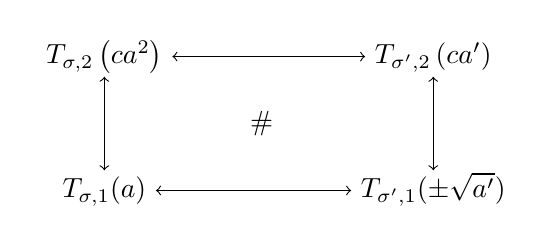
\begin{tikzpicture}[description/.style={fill=white,inner sep=2pt}]
\matrix (m) [matrix of math nodes, row sep=1em,column sep=2.5em,%
text height=1.5ex, text depth=0.25ex]
{ T_{\sigma,2}\left(ca^2\right) & & T_{\sigma',2}\left(ca'\right) \\
&\#&\\
T_{\sigma,1}(a) & &T_{\sigma',1}(\pm\sqrt{a'}) \\ };
\path[<->](m-1-1) edge node[auto] {$$}(m-1-3);
\path[<->](m-3-1) edge node[anchor=north]{$$}(m-3-3);
\path[<->](m-3-1) edge node[auto]{$$}(m-1-1);
\path[<->](m-1-3) edge node[auto]{$$}(m-3-3);
\end{tikzpicture}
\end{figure}
Therefore we determined $P_1(T_1,T_2)$ and $P_2(T_1,T_2)$, where $T_1$ and
$T_2$ are real subtypes of the the main type $\widetilde Y_r$, using the
structure of the equivalence classes of the $Y_{r,s}$ singularities.

\begin{example}\label{tab:counter_example_Yr}
Let $T_1$ be a real subtype of $\widetilde Y_8$. Taking
Diagram~\ref{Yr_commuting_diagram} into account it follows that
$(a,-a)\in P_2(T_1,T_1)$, $a\in\R$. Hence $\phi(T_1(a))=T_1(-a)$. Considering
the transformations in $S_1$ and $S_2$ in Theorem \ref{tab:sufficient_sets}, it
is clear that $\phi\not\in S_1$ and $\phi\not\in S_2$, i.e.~$S_1$ and $S_2$ are
not sufficient sets of $\C$-transformations preserving $\C$ or $\R$ for $T_1$
and $T_1$.
\end{example}

Let $T_1$ and $T_2$ be real subtypes of $\widetilde Y_r$ and let $a\in\R$. We
now consider $P_3(T_1,T_2)$. It is clear that $P_3(T_1,T_2)=\varnothing$, if
$T_1$ and $T_2$ are not of the same subtype. Furthermore, it is clear that
$P_3(T_1,T_1)\subset P_2(T_1,T_1)\subset\{(a,-a)\mid a\in\R\}$ and that
$(a,-a)\in P_3(T_1,T_1)$, if $r$ is odd. Since $T_1(a)$ is finite determinate,
$f(x)=c^4+c^2x^2+|a|x^r$, $c\in\R$ has only positive values, while
$g(x)=c^4+c^2x^2-|a|x^r$, has negative values, it follows that
$(a,-a)\not\in P_3(T_1,T_1)$, if $r$ is even.

\begin{remark}
Considering $P_3(T_1,T_2)$, where $T_1$ and $T_2$ are real subtypes of
$\widetilde Y_r$, it follows that $S_1$ is a sufficient set of
$\R$-transformations preserving $\R$ for real subtypes of $\widetilde Y_r$.
\end{remark}


\section{Results}\label{sec:results}

In this section we present the sets $P_1,P_2,P_3$ in table form for every
unimodal real singularity type up to corank 2.

\begin{theorem}\label{thm:X9}
The structure of the equivalence classes of the $X_9$ singularities is as shown
in Table~\ref{tab:X9_equivalences} where for $j = 1, \ldots, 6$ and
$\rho, \sigma \in \{1, i\}$, the function $f_j^{\rho, \sigma}$ is defined as
follows:
\begin{align*}
f_1^{\rho, \sigma}(a) &:= +\rho \sigma \cdot a \,, &
f_3^{\rho, \sigma}(a) &:= \frac{+2\sigma a+12\rho\sigma}{a-2\rho} \,, &
f_5^{\rho, \sigma}(a) &:= \frac{-2\sigma a+12\rho\sigma}{a+2\rho} \,, \\
f_2^{\rho, \sigma}(a) &:= -\rho \sigma \cdot a \,, &
f_4^{\rho, \sigma}(a) &:= \frac{+2\sigma a-12\rho\sigma}{a+2\rho} \,, &
f_6^{\rho, \sigma}(a) &:= \frac{-2\sigma a-12\rho\sigma}{a-2\rho} \,.
\end{align*}

Furthermore, we use the following notations:
\begin{align*}
\C'  &:= \C \setminus \{ -2, 2\} \,, &
\R'  &:= \R \setminus \{ -2, 2\} \,, &
\C'' &:= \C \setminus \{ -2i, 2i\} \,.
\end{align*}

\newcommand{\specialvrule}{\rule[-1.8ex]{0pt}{5ex}}
\begin{table}[htbp]
\centering
\caption{$P_1$, $P_2$ and $P_3$ for the $X_9$ singularities}
\label{tab:X9_equivalences}
\begin{tabular}{|c|c||c|c|c|}
\hline

$T_1$ & $T_2$ & $P_1(T_1, T_2)$ & $P_2(T_1, T_2)$ & $P_3(T_1, T_2)$ \\
\hline\hline

$X_9^{++}$ & $X_9^{++}$ &
\multirow{6}{*}{$\Gamma_{\C'}\left(f_1^{1,1}, \ldots, f_6^{1,1}\right)$} &
\multirow{6}{*}{$\Gamma_{\R'}\left(f_1^{1,1}, \ldots, f_6^{1,1}\right)$} &
\begin{tabular}[x]{@{}l@{}}
    $\phantom{\cup}\; \Gamma_{\R'}\left(f_1^{1,1}\right)$\specialvrule \\
    $\cup\; \Gamma_{\R^{>-2}}\left(f_5^{1,1}\right)$\specialvrule
\end{tabular}
\\ \cline{1-2}\cline{5-5}

$X_9^{--}$ & $X_9^{--}$ &&&
\begin{tabular}[x]{@{}l@{}}
    $\phantom{\cup}\; \Gamma_{\R'}\left(f_1^{1,1}\right)$\specialvrule \\
    $\cup\; \Gamma_{\R^{<2}}\left(f_3^{1,1}\right)$\specialvrule
\end{tabular}
\\ \cline{1-2}\cline{5-5}

$X_9^{++}$ & $X_9^{--}$ &&&
$\Gamma_{\R^{<-2}}\left(f_4^{1,1}\right)$\specialvrule
\\ \cline{1-2}\cline{5-5}

$X_9^{--}$ & $X_9^{++}$ &&&
$\Gamma_{\R^{>2}}\left(f_6^{1,1}\right)$\specialvrule
\\ \hline


$X_9^{+-}$ & $X_9^{+-}$ &
\multirow{4}{*}{$\Gamma_{\C''}\left(f_1^{i,i}, \ldots, f_6^{i,i}\right)$} &
\multirow{4}{*}{$\Gamma_{\R}\left(f_1^{1,1}, f_2^{1,1}\right)$} &
\multirow{4}{*}{$\Gamma_{\R}\left(f_1^{1,1}\right)$} \\ \cline{1-2}

$X_9^{-+}$ & $X_9^{-+}$ &&& \\ \cline{1-2}

$X_9^{+-}$ & $X_9^{-+}$ &&& \\ \cline{1-2}

$X_9^{-+}$ & $X_9^{+-}$ &&& \\ \hline


$X_9^{++}$ & $X_9^{+-}$ &
\multirow{4}{*}{$\Gamma_{\C'}\left(f_1^{1,i}, \ldots, f_6^{1,i}\right)$} &
\multirow{4}{*}{$\{(-6,0), (0,0), (6,0)\}$} &
\multirow{4}{*}{$\varnothing$} \\ \cline{1-2}

$X_9^{++}$ & $X_9^{-+}$ &&& \\ \cline{1-2}

$X_9^{--}$ & $X_9^{+-}$ &&& \\ \cline{1-2}

$X_9^{--}$ & $X_9^{-+}$ &&& \\ \hline


$X_9^{+-}$ & $X_9^{++}$ &
\multirow{4}{*}{$\Gamma_{\C''}\left(f_1^{i,1}, \ldots, f_6^{i,1}\right)$} &
\multirow{4}{*}{$\{(0,-6), (0,0), (0,6)\}$} &
\multirow{4}{*}{$\varnothing$} \\ \cline{1-2}

$X_9^{-+}$ & $X_9^{++}$ &&& \\ \cline{1-2}

$X_9^{+-}$ & $X_9^{--}$ &&& \\ \cline{1-2}

$X_9^{-+}$ & $X_9^{--}$ &&& \\ \hline
\end{tabular}
\end{table}

\end{theorem}


\begin{theorem}\label{tab:J10_equivalences_2}\label{thm:J10}
The structure of the equivalence classes of the $J_{10}$ singularities is as
shown in Table~\ref{tab:J10_equivalences} where for $j = 1, \ldots, 6$ and
$\rho, \sigma \in \{-1, +1\}$, the function $f_j^{\rho, \sigma}$ is defined as
follows:
\begin{align*}
f_1^{\rho, \sigma}(a) &:= +\sqrt{\rho \sigma} \cdot a \,, \\
f_2^{\rho, \sigma}(a) &:= -\sqrt{\rho \sigma} \cdot a \,, \\
f_3^{\rho, \sigma}(a)
&:= + \sqrt{\frac{-\rho \sigma (a^2-\rho \cdot 4) (a^2-\rho \cdot 9)
    + a (a^2-\rho \cdot 3) \sqrt{a^2-\rho \cdot 4}}{2(a^2-\rho \cdot 4)}}\,, \\
f_4^{\rho, \sigma}(a)
&:= - \sqrt{\frac{-\rho \sigma (a^2-\rho \cdot 4) (a^2-\rho \cdot 9)
    + a (a^2-\rho \cdot 3) \sqrt{a^2-\rho \cdot 4}}{2(a^2-\rho \cdot 4)}}\,, \\
f_5^{\rho, \sigma}(a)
&:= + \sqrt{\frac{-\rho \sigma (a^2-\rho \cdot 4) (a^2-\rho \cdot 9)
    - a (a^2-\rho \cdot 3) \sqrt{a^2-\rho \cdot 4}}{2(a^2-\rho \cdot 4)}}\,, \\
f_6^{\rho, \sigma}(a)
&:= - \sqrt{\frac{-\rho \sigma (a^2-\rho \cdot 4) (a^2-\rho \cdot 9)
    - a (a^2-\rho \cdot 3) \sqrt{a^2-\rho \cdot 4}}{2(a^2-\rho \cdot 4)}}\,.
\end{align*}

In each case, $\rho$ and $\sigma$ are given by
\begin{align*}
\rho &:=
\begin{cases}
    +1, &\text{if } T_1 = J_{10}^+ \,, \\
    -1, &\text{if } T_1 = J_{10}^- \,, \\
\end{cases}
&\sigma &:=
\begin{cases}
    +1, &\text{if } T_2 = J_{10}^+ \,, \\
    -1, &\text{if } T_2 = J_{10}^- \,. \\
\end{cases}
\end{align*}

Furthermore, we use the following notations:
\begin{align*}
\C'  &:= \C \setminus \{ -2, 2\} \,, &
\R'  &:= \R \setminus \{ -2, 2\} \,, \\
I_1 &:= \left] {\textstyle\frac{3}{\sqrt{2}}}, \infty \right[ \subset \R \,, &
I_2 &:= \left] 2, {\textstyle\frac{3}{\sqrt{2}}} \right[ \subset \R      \,, \\
I_3 &:= \left] {\textstyle-\frac{3}{\sqrt{2}}}, -2 \right[ \subset \R    \,, &
I_4 &:= \left] -\infty, {\textstyle-\frac{3}{\sqrt{2}}} \right[ \subset \R \,.
\end{align*}

\newcommand{\specialvrule}{\rule[-1.9ex]{0pt}{4.8ex}}
\begin{table}[htbp]
\centering
\caption{$P_1$, $P_2$ and $P_3$ for the $J_{10}$ singularities}
\label{tab:J10_equivalences}
\begin{tabular}{|c|c||c|c|c|}
\hline

$T_1$ & $T_2$ & $P_1(T_1, T_2)$ & $P_2(T_1, T_2)$ & $P_3(T_1, T_2)$ \\
\hline\hline

$J_{10}^+$ & $J_{10}^+$ &
$\Gamma_{\C'}\left(f_1^{\rho,\sigma}, \ldots, f_6^{\rho,\sigma}\right)$ &
\begin{tabular}[x]{@{}l@{}}
    $\phantom{\cup}\; \Gamma_{\R'}\left(f_1^{\rho,\sigma},
        f_2^{\rho,\sigma}\right)$ \\
    $\cup\; \Gamma_{\R^{>+2}}\left(f_3^{\rho,\sigma},
        f_4^{\rho,\sigma}\right)$ \\
    $\cup\; \Gamma_{\R^{<-2}}\left(f_5^{\rho,\sigma},
        f_6^{\rho,\sigma}\right)$ \\
    $\cup \left\{\left(0, \frac{-3}{\sqrt{2}}\right),
        \left(0, \frac{+3}{\sqrt{2}}\right)\right\}$\specialvrule \\
    $\cup \left\{\left(\frac{-3}{\sqrt{2}}, 0\right),
        \left(\frac{+3}{\sqrt{2}}, 0\right)\right\}$\specialvrule \\
\end{tabular} &
\begin{tabular}[x]{@{}l@{}}
    $\phantom{\cup}\; \Gamma_{\R'}\left(f_1^{\rho,\sigma}\right)$ \\
    $\cup\; \Gamma_{\R^{>+2}}\left(f_4^{\rho,\sigma}\right)$ \\
    $\cup\; \Gamma_{\R^{<-2}}\left(f_5^{\rho,\sigma}\right)$ \\
\end{tabular} \\
\hline

$J_{10}^-$ & $J_{10}^-$ &
$\Gamma_{\C}\left(f_1^{\rho,\sigma}, \ldots, f_6^{\rho,\sigma}\right)$ &
$\Gamma_{\R}\left(f_1^{\rho,\sigma}, f_2^{\rho,\sigma}\right)$ &
$\Gamma_{\R}\left(f_1^{\rho,\sigma}\right)$ \\
\hline

$J_{10}^+$ & $J_{10}^-$ &
$\Gamma_{\C'}\left(f_1^{\rho,\sigma}, \ldots, f_6^{\rho,\sigma}\right)$ &
\begin{tabular}[x]{@{}l@{}}
    $\phantom{\cup}\; \{(0, 0)\}$ \\
    $\cup\; \Gamma_{\R^{>+2}}\left(f_3^{\rho,\sigma},
        f_4^{\rho,\sigma}\right)$ \\
    $\cup\; \Gamma_{\R^{<-2}}\left(f_5^{\rho,\sigma},
        f_6^{\rho,\sigma}\right)$ \\
\end{tabular} &
\begin{tabular}[x]{@{}l@{}}
    $\phantom{\cup}\; \Gamma_{I_1} \left(f_3^{\rho,\sigma}\right)$ \\
    $\cup\; \Gamma_{I_2} \left(f_4^{\rho,\sigma}\right)$ \\
    $\cup\; \Gamma_{I_3} \left(f_5^{\rho,\sigma}\right)$ \\
    $\cup\; \Gamma_{I_4} \left(f_6^{\rho,\sigma}\right)$ \\
    $\cup \left\{\left(\frac{-3}{\sqrt{2}}, 0\right),
        \left(\frac{+3}{\sqrt{2}}, 0\right)\right\}$\specialvrule \\
\end{tabular} \\
\hline

$J_{10}^-$ & $J_{10}^+$ &
$\Gamma_{\C}\left(f_1^{\rho,\sigma}, \ldots, f_6^{\rho,\sigma}\right)$ &
\begin{tabular}[x]{@{}l@{}}
    $\phantom{\cup}\; \{(0, 0)\}$ \\
    $\cup\; \Gamma_{\R}\left(f_3^{\rho,\sigma}, \ldots,
        f_6^{\rho,\sigma}\right)$ \\
\end{tabular} &
\begin{tabular}[x]{@{}l@{}}
    $\phantom{\cup}\; \Gamma_{\R^{>0}}\left(f_3^{\rho,\sigma},
        f_6^{\rho,\sigma}\right)$ \\
    $\cup\; \Gamma_{\R^{<0}}\left(f_4^{\rho,\sigma},
        f_5^{\rho,\sigma}\right)$ \\
    $\cup \left\{\left(0, \frac{-3}{\sqrt{2}}\right),
        \left(0, \frac{+3}{\sqrt{2}}\right)\right\}$\specialvrule \\
\end{tabular} \\
\hline

\end{tabular}
\end{table}

\end{theorem}


\begin{theorem}
The structure of the equivalence classes of the $J_{10+k}$
singularities is as shown in Table~\ref{tab:J10+k_equivalences} where in each
case, $l$ and $s$ are given by
\begin{align*}
l &:= \frac{6}{\gcd(6,k)}, \text{ and} \\
s &:=
\begin{cases}
  +1, &\text{if } k \equiv 2 \pmod{4}, \\
  -1, &\text{else.}
\end{cases}
\end{align*}

\begin{table}[htbp]
\centering
\caption{$P_1$, $P_2$ and $P_3$ for the $J_{10+k}$ singularities}
\label{tab:J10+k_equivalences}
\begin{tabular}{|c|c||c|c|c|}
\hline

$T_1$ & $T_2$ & $P_1(T_1, T_2)$ & $P_2(T_1, T_2)$ & $P_3(T_1, T_2)$ \\
\hline\hline

$J_{10+k}^+$ & $J_{10+k}^+$ &
\multirow{2}{*}{$C(X^l-1)$} &
\multirow{2}{*}{$R(X^l-1)$} &
\multirow{2}{*}{$R(X^l-1)$} \\
\cline{1-2}

$J_{10+k}^-$ & $J_{10+k}^-$ &&& \\
\hline

$J_{10+k}^+$ & $J_{10+k}^-$ &
\multirow{2}{*}{$C(X^l-s)$} &
\multirow{2}{*}{$R(X^l-s)$} &
\multirow{2}{*}{$\varnothing$} \\
\cline{1-2}

$J_{10+k}^-$ & $J_{10+k}^+$ &&& \\
\hline

\end{tabular}
\end{table}

\end{theorem}


\begin{theorem}
The structure of the equivalence classes of the $X_{9+k}$
singularities is as shown in Table~\ref{tab:X9+k_equivalences} where in each
case, $l$ and $s$ are given by
\begin{align*}
l &:= \frac{4}{\gcd(4,k)}, \text{ and} \\
s &:=
\begin{cases}
  +1, &\text{if } k \equiv 4 \pmod{8}, \\
  -1, &\text{else.}
\end{cases}
\end{align*}

\begin{table}[htbp]
\centering
\caption{$P_1$, $P_2$ and $P_3$ for the $X_{9+k}$ singularities}
\label{tab:X9+k_equivalences}
\begin{tabular}{|c|c||c|c|c|}
\hline

$T_1$ & $T_2$ & $P_1(T_1, T_2)$ & $P_2(T_1, T_2)$ & $P_3(T_1, T_2)$ \\
\hline\hline

$X_{9+k}^{++}$ & $X_{9+k}^{++}$ &
\multirow{4}{*}{$C(X^l-1)$} &
\multirow{4}{*}{$R(X^l-1)$} &
\multirow{4}{*}{$R(X^{k+1}-1)$} \\
\cline{1-2}

$X_{9+k}^{+-}$ & $X_{9+k}^{+-}$ &&& \\ \cline{1-2}
$X_{9+k}^{-+}$ & $X_{9+k}^{-+}$ &&& \\ \cline{1-2}
$X_{9+k}^{--}$ & $X_{9+k}^{--}$ &&& \\ \hline


$X_{9+k}^{++}$ & $X_{9+k}^{+-}$ &
\multirow{4}{*}{$C(X^l-1)$} &
\multirow{4}{*}{$R(X^l-1)$} &
\multirow{4}{*}{$\varnothing$} \\
\cline{1-2}

$X_{9+k}^{+-}$ & $X_{9+k}^{++}$ &&& \\ \cline{1-2}
$X_{9+k}^{-+}$ & $X_{9+k}^{--}$ &&& \\ \cline{1-2}
$X_{9+k}^{--}$ & $X_{9+k}^{-+}$ &&& \\ \hline


$X_{9+k}^{++}$ & $X_{9+k}^{-+}$ &
\multirow{4}{*}{$C(X^l-s)$} &
\multirow{4}{*}{$R(X^l-s)$} &
\multirow{4}{*}{$\varnothing$} \\
\cline{1-2}

$X_{9+k}^{+-}$ & $X_{9+k}^{--}$ &&& \\ \cline{1-2}
$X_{9+k}^{-+}$ & $X_{9+k}^{++}$ &&& \\ \cline{1-2}
$X_{9+k}^{--}$ & $X_{9+k}^{+-}$ &&& \\ \hline


$X_{9+k}^{++}$ & $X_{9+k}^{--}$ &
\multirow{4}{*}{$C(X^l-s)$} &
\multirow{4}{*}{$R(X^l-s)$} &
\multirow{4}{*}{$\varnothing$} \\
\cline{1-2}

$X_{9+k}^{+-}$ & $X_{9+k}^{-+}$ &&& \\ \cline{1-2}
$X_{9+k}^{-+}$ & $X_{9+k}^{+-}$ &&& \\ \cline{1-2}
$X_{9+k}^{--}$ & $X_{9+k}^{++}$ &&& \\ \hline

\end{tabular}
\end{table}

\end{theorem}


\begin{theorem}
The structure of the equivalence classes of the $Y_{r,s}$ singularities is as
shown in Table~\ref{tab:Yrs_equivalences} where in each case, $l$, $s_1$ and
$s_2$ are given by
\begin{align*}
l &:= \frac{r}{\gcd(r,s)} \cdot \gcd(2, r+1, s+1) \,, \\
s_1 &:=
\begin{cases}
  +1, &\text{if } r \equiv 0 \pmod{4} \text{ or } s \equiv 0 \pmod{4}, \\
  -1, &\text{else,}
\end{cases} \\
s_2 &:=
\begin{cases}
  +1, &\text{if } r \not\equiv 0 \pmod{2}
      \text{ or } \frac{s}{\gcd(r,s)} \equiv 0 \pmod{2}, \\
  -1, &\text{else.}
\end{cases}
\end{align*}

In the special case where $r = s$, additional equivalences occur. They are
listed in Table~\ref{tab:Yrr_equivalences}.

\begin{table}[htbp]
\centering
\caption{$P_1$, $P_2$ and $P_3$ for the $Y_{r,s}$ singularities}
\label{tab:Yrs_equivalences}
\begin{tabular}{|c|c||c|c|c|}
\hline

$T_1$ & $T_2$ & $P_1(T_1, T_2)$ & $P_2(T_1, T_2)$ & $P_3(T_1, T_2)$ \\
\hline\hline

$Y_{r,s}^{++}$ & $Y_{r,s}^{++}$ &
\multirow{4}{*}{$C(X^l-1)$} &
\multirow{4}{*}{$R(X^l-1)$} &
\multirow{4}{*}{$R(X^{s+1}-1)$}
\\ \cline{1-2}

$Y_{r,s}^{-+}$ & $Y_{r,s}^{-+}$ &&&
\\ \cline{1-2}

$Y_{r,s}^{+-}$ & $Y_{r,s}^{+-}$ &&&
\\ \cline{1-2}

$Y_{r,s}^{--}$ & $Y_{r,s}^{--}$ &&&
\\ \hline


$Y_{r,s}^{++}$ & $Y_{r,s}^{-+}$ &
\multirow{4}{*}{$C(X^l-s_1)$} &
\multirow{4}{*}{$R(X^l-s_1)$} &
\multirow{4}{*}{$\varnothing$}
\\ \cline{1-2}

$Y_{r,s}^{-+}$ & $Y_{r,s}^{++}$ &&&
\\ \cline{1-2}

$Y_{r,s}^{+-}$ & $Y_{r,s}^{--}$ &&&
\\ \cline{1-2}

$Y_{r,s}^{--}$ & $Y_{r,s}^{+-}$ &&&
\\ \hline


$Y_{r,s}^{++}$ & $Y_{r,s}^{+-}$ &
\multirow{4}{*}{$C(X^l-s_2)$} &
\multirow{4}{*}{$R(X^l-s_2)$} &
\multirow{4}{*}{$\begin{cases}
  R(X^l-s_2),  &\text{if } r \not\equiv 0 \pmod{2} \\
  \varnothing, &\text{if } r \equiv 0 \pmod{2}
\end{cases}$}
\\ \cline{1-2}

$Y_{r,s}^{-+}$ & $Y_{r,s}^{--}$ &&&
\\ \cline{1-2}

$Y_{r,s}^{+-}$ & $Y_{r,s}^{++}$ &&&
\\ \cline{1-2}

$Y_{r,s}^{--}$ & $Y_{r,s}^{-+}$ &&&
\\ \hline


$Y_{r,s}^{++}$ & $Y_{r,s}^{--}$ &
\multirow{4}{*}{$C(X^l-s_1 s_2)$} &
\multirow{4}{*}{$R(X^l-s_1 s_2)$} &
\multirow{4}{*}{$\varnothing$}
\\ \cline{1-2}

$Y_{r,s}^{-+}$ & $Y_{r,s}^{+-}$ &&&
\\ \cline{1-2}

$Y_{r,s}^{+-}$ & $Y_{r,s}^{-+}$ &&&
\\ \cline{1-2}

$Y_{r,s}^{--}$ & $Y_{r,s}^{++}$ &&&
\\ \hline

\end{tabular}
\end{table}

\begin{table}[htbp]
\centering
\caption{Additional equivalences for the $Y_{r,s}$ singularities in the
special case $r = s$}
\label{tab:Yrr_equivalences}
\begin{tabular}{|c|c||c|}
\hline

$T_1$ & $T_2$ & $P_3(T_1, T_2)$ \\
\hline\hline

$Y_{r,s}^{++}$ & $Y_{r,s}^{+-}$ &
\multirow{2}{*}{$\begin{cases}
  R(X+1),      &\!\text{if } r \equiv 0 \pmod{2} \text{ and } a < 0 \\
  \varnothing, &else
\end{cases}$}
\\ \cline{1-2}

$Y_{r,s}^{-+}$ & $Y_{r,s}^{--}$ &
\\ \hline

$Y_{r,s}^{+-}$ & $Y_{r,s}^{++}$ &
\multirow{2}{*}{$\begin{cases}
  R(X+1),      &\!\text{if } r \equiv 0 \pmod{2} \text{ and } a > 0 \\
  \varnothing, &else
\end{cases}$}
\\ \cline{1-2}

$Y_{r,s}^{--}$ & $Y_{r,s}^{-+}$ &
\\ \hline

\end{tabular}
\end{table}

\end{theorem}


\begin{theorem}
The structure of the equivalence classes of the $\tY_r$ singularities is as
shown in Table~\ref{tab:tYr_equivalences} where in each case, $l$ and $s$ are
given by
\begin{align*}
l &:= 2\cdot{\gcd(2, r+1)}, \text{ and} \\
s &:=
\begin{cases}
  +1, &\text{if } r \equiv 0 \pmod{4}, \\
  -1, &\text{else.}
\end{cases}
\end{align*}

\begin{table}[htbp]
\centering
\caption{$P_1$, $P_2$ and $P_3$ for the $\tY_r$ singularities}
\label{tab:tYr_equivalences}
\begin{tabular}{|c|c||c|c|c|}
\hline

$T_1$ & $T_2$ & $P_1(T_1, T_2)$ & $P_2(T_1, T_2)$ & $P_3(T_1, T_2)$ \\
\hline\hline

$\tY_r^+$ & $\tY_r^+$ &
\multirow{2}{*}{$C(X^l-1)$} &
\multirow{2}{*}{$R(X^2-1)$} &
\multirow{2}{*}{$\begin{cases}
  R(X^2-1), &\text{if } r \equiv 1 \pmod{2} \\
  R(X-1),   &\text{if } r \equiv 0 \pmod{2}
\end{cases}$} \\
\cline{1-2}

$\tY_r^-$ & $\tY_r^-$ &
&
&
\\
\hline

$\tY_r^+$ & $\tY_r^-$ &
\multirow{2}{*}{$C(X^l-s)$} &
\multirow{2}{*}{$R(X^l-s)$} &
\multirow{2}{*}{$\varnothing$} \\
\cline{1-2}

$\tY_r^-$ & $\tY_r^+$ &
&
&
\\
\hline

\end{tabular}
\end{table}

\end{theorem}


\begin{theorem}
The structure of the equivalence classes of the exceptional unimodal
singularities is as shown in Table~\ref{tab:exceptional_equivalences}.

\begin{table}[htbp]
\centering
\caption{$P_1$, $P_2$ and $P_3$ for the exceptional unimodal singularities}
\label{tab:exceptional_equivalences}
\begin{tabular}{|c|c||c|c|c|}
\hline
$T_1$ & $T_2$ & $P_1(T_1, T_2)$ & $P_2(T_1, T_2)$ & $P_3(T_1, T_2)$ \\
\hline\hline
$E_{12}$   & $E_{12}$   & $C(X^{21}-1)$ & $R(X-1)$      & $R(X-1)$ \\
\hline
$E_{13}$   & $E_{13}$   & $C(X^{15}-1)$ & $R(X-1)$      & $R(X-1)$ \\
\hline
$E_{14}^+$ & $E_{14}^+$ & $C(X^{12}-1)$ & $R(X^2-1)$    & $R(X-1)$ \\
\hline
$E_{14}^-$ & $E_{14}^-$ & $C(X^{12}-1)$ & $R(X^2-1)$    & $R(X-1)$ \\
\hline
$E_{14}^+$ & $E_{14}^-$ & $C(X^{12}+1)$ & $\varnothing$ & $\varnothing$ \\
\hline
$E_{14}^-$ & $E_{14}^+$ & $C(X^{12}+1)$ & $\varnothing$ & $\varnothing$ \\
\hline
$Z_{11}$   & $Z_{11}$   & $C(X^{15}-1)$ & $R(X-1)$      & $R(X-1)$ \\
\hline
$Z_{12}$   & $Z_{12}$   & $C(X^{11}-1)$ & $R(X-1)$      & $R(X-1)$ \\
\hline
$Z_{13}^+$ & $Z_{13}^+$ & $C(X^9-1)$    & $R(X-1)$      & $R(X-1)$ \\
\hline
$Z_{13}^-$ & $Z_{13}^-$ & $C(X^9-1)$    & $R(X-1)$      & $R(X-1)$ \\
\hline
$Z_{13}^+$ & $Z_{13}^-$ & $C(X^9+1)$    & $R(X+1)$      & $\varnothing$ \\
\hline
$Z_{13}^-$ & $Z_{13}^+$ & $C(X^9+1)$    & $R(X+1)$      & $\varnothing$ \\
\hline
$W_{12}^+$ & $W_{12}^+$ & $C(X^{10}-1)$ & $R(X^2-1)$    & $R(X-1)$ \\
\hline
$W_{12}^-$ & $W_{12}^-$ & $C(X^{10}-1)$ & $R(X^2-1)$    & $R(X-1)$ \\
\hline
$W_{12}^+$ & $W_{12}^-$ & $C(X^{10}+1)$ & $\varnothing$ & $\varnothing$ \\
\hline
$W_{12}^-$ & $W_{12}^+$ & $C(X^{10}+1)$ & $\varnothing$ & $\varnothing$ \\
\hline
$W_{13}^+$ & $W_{13}^+$ & $C(X^8-1)$    & $R(X^2-1)$    & $R(X-1)$ \\
\hline
$W_{13}^-$ & $W_{13}^-$ & $C(X^8-1)$    & $R(X^2-1)$    & $R(X-1)$ \\
\hline
$W_{13}^+$ & $W_{13}^-$ & $C(X^8+1)$    & $\varnothing$ & $\varnothing$ \\
\hline
$W_{13}^-$ & $W_{13}^+$ & $C(X^8+1)$    & $\varnothing$ & $\varnothing$ \\
\hline
\end{tabular}
\end{table}

\end{theorem}


\section{Acknowledgements}

We would like to thank Claus Fieker, Gert-Martin Greuel, and Gerhard Pfister
for many fruitful discussions.


\begin{thebibliography}{99}
\bibitem{AVG1985} Arnold, V.I.; Gusein-Zade, S.M.; Varchenko, A.N.:
Singularities of Differential Maps. Vol.~I, Birkh\"auser (1985).
\bibitem{A1975} Arnold, V.I.:
\textit{Normal form of functions near degenerate critical points.},
Russian Mth. Surveys 29 ii (1975), 10-50.
\bibitem{DGPS}
Decker, W.; Greuel, G.-M.; Pfister, G.; Sch{\"o}nemann, H.:
\newblock {\sc Singular} {3-1-5} --- {A} computer algebra system for polynomial
computations.
\newblock {http://www.singular.uni-kl.de} (2012).
\bibitem{Kruger} Kr\"uger, K.: Klassifikation von
Hyperfl\"agensingularit\"aten, Diploma Thesis (1997).
\bibitem{GLS2007}Greuel, G.-M.; Lossen, C.; Shustin E.:
Introduction to Singularities and Deformations, Springer, Berlin (2007).
\bibitem{GP2008} Greuel G.-M.; Pfister G.;
A Singular introduction to Commutative Algebra, 2nd Ed., Springer,
Berlin (2008).
\bibitem{classify}
Kr\"uger, K.:
{\tt classify.lib}. {A} {\sc Singular} {3-1-5} library for classifying isolated
hypersurface singularities w.r.t. right equivalence, based on the determinator
of singularities by V.I. Arnold (2012).
\bibitem{realclassify}
Marais, M. and Steenpass, A.:
{\tt realclassify.lib}. {A} {\sc Singular} {3-1-5} library for classifying
isolated hypersurface singularities over the reals w.r.t. right equivalence,
based on the determinator of singularities by V.I. Arnold. This library is
based on classify.lib by Kai Kr\"uger, but handles the real case, while
classify.lib does the complex classification (2012).

\bibitem{MS2013}Marais, M.S.; Steenpa\ss, A.:
The classification of real singularities using \textsc{Singular}. Part I:
Splitting Lemma and Simple Singularities. (2013)

\bibitem{grobcov}
Montes, A. and Sch\"onemann, H.:
{\tt grobcov.lib}. {A} {\sc Singular} {3-1-6} library for Gr\"obner Covers of
of Parametric Ideals (2013).

\bibitem{primdec} Pfister, G.; Decker, W.; Schoenemann, H.; Laplagne, S.:
{\tt primdec.lib}. {A} {\sc Singular} {3-1-5} library for Primary Decomposition
and Radical of Ideals (2012).
\bibitem{PdJ2000}
Pfister, G.; De Jongh, T.:
Local analytic Geometry, Amer. Math. Soc. (2000)
\bibitem{Siersma} Siersma D.: Classification and deformation of Singularities,
disertation, University of Amsterdam (1974).
\bibitem{roots}
Tobis, A.:
{\tt rootsur.lib}. {A} {\sc Singular} {3-1-5} library for Counting number of
real roots of univariate polynomial (2012).
\bibitem{solve.lib} Wenk, M.: {\tt solve.lib}. Pohl, W.:
{A} {\sc Singular} {3-1-5} library for Complex Solving of Polynomial Systems
(2012).

\end{thebibliography}

\end{document}
